% IEEE Design & Test feature article, laid out after the D&T house pattern
% (department tag, sans-serif title and headings, unnumbered sentence-case
% sections, small-caps lead-in, unheaded closing with end mark, "References"
% and bios without heading, "Direct questions" line). CEDA author guidelines
% take precedence: <= 5,000 words incl. references and bios (200 per figure or
% table), <= 12 references, title <= 9 words, introduction 1-5 paragraphs,
% conclusion 1-2 paragraphs, bios with position, degree, <= 3 interests, e-mail.
% Author manuscript for IEEE Design & Test (SI: SBCCI 2026). D&T publishes no
% template; production applies the magazine layout after acceptance. This file
% follows the CEDA author guidelines (<= 5,000 words incl. references and bios,
% 200 per figure/table; <= 12 references; title <= 9 words; opening 1-5
% paragraphs without an "Introduction" heading; conclusion 1-2 paragraphs;
% bios with position, degree, <= 3 interests, e-mail) and the structure of
% published D&T features (unnumbered sentence-case headings).
\documentclass[10pt,twocolumn]{article}
\usepackage[utf8]{inputenc}
\usepackage[T1]{fontenc}
\usepackage{mathptmx}
\usepackage[letterpaper,top=0.75in,bottom=0.85in,left=0.7in,right=0.7in,columnsep=0.24in]{geometry}
\usepackage{graphicx,booktabs,amsmath,xcolor,array,cite,url,textcomp}
\usepackage[shortlabels]{enumitem}
\graphicspath{{figures/}}
\usepackage[font=footnotesize,labelfont=bf,labelsep=period,skip=4pt]{caption}
\usepackage{titlesec,fancyhdr}
\setcounter{secnumdepth}{0}
\titleformat{\section}{\normalfont\large\bfseries\color{black!80}}{}{0pt}{}
\titlespacing*{\section}{0pt}{9pt plus 2pt}{3pt}
\renewcommand{\figurename}{Figure}
\renewcommand{\tablename}{Table}
\captionsetup[table]{position=top}
\pagestyle{fancy}\fancyhf{}
\fancyhead[L]{\footnotesize\itshape IEEE Design \& Test --- Special Issue: SBCCI 2026}
\fancyhead[R]{\footnotesize\itshape Alencar et al.: When Can an On-Chip Sensor See Aging Under Burn-In?}
\fancyfoot[C]{\footnotesize\thepage}
\renewcommand{\headrulewidth}{0.3pt}
\setlength{\parskip}{0pt}
\setlist{itemsep=1pt,parsep=0pt}
\definecolor{pid}{HTML}{1F5FBF}\definecolor{bb}{HTML}{D9661F}
\newcommand{\Tmin}{T_{\min}}
\newcommand{\tint}{\tau_{\mathrm{int}}}
% units without siunitx (keeps the source buildable on TeX Live 2020)
\newcommand{\degC}{\,\textdegree C}
\newcommand{\unit}[1]{\,\mathrm{#1}}
\newcommand{\mcnth}{\,m\,cnt/h}
\newcommand{\dttitle}{When Can an On-Chip Sensor See Aging Under Burn-In?}
\hyphenation{Arrhe-nius}
% every result printed below comes from analysis/ through these macros
% AUTO-GENERATED by analysis/derive.py -- do not edit by hand.
% Every number printed in the manuscript comes from one of these macros.
\newcommand{\vAFBB}{31.1}
\newcommand{\vAFBBlong}{31.8}
\newcommand{\vAFPID}{51.3}
\newcommand{\vAFRCA}{78.1}
\newcommand{\vAFdevBB}{$-$33}
\newcommand{\vAFdevPID}{12}
\newcommand{\vAFfullBB}{31.1}
\newcommand{\vAFfullPID}{51.3}
\newcommand{\vAFratio}{1.65}
\newcommand{\vAFratioFull}{1.65}
\newcommand{\vAFratioFullHi}{1.90}
\newcommand{\vAFratioFullLo}{1.43}
\newcommand{\vAFratioHi}{1.90}
\newcommand{\vAFratioHiOne}{1.9}
\newcommand{\vAFratioLo}{1.43}
\newcommand{\vAFratioLoOne}{1.4}
\newcommand{\vAFratioMeanOnly}{1.66}
\newcommand{\vAFratioSPadj}{1.40}
\newcommand{\vAFratioSPgain}{1.35}
\newcommand{\vAdevTwoBB}{0.88}
\newcommand{\vAdevTwoBBlong}{0.87}
\newcommand{\vAdevTwoPID}{0.68}
\newcommand{\vAdevTwoRCA}{0.71}
\newcommand{\vAdevTwoRatio}{1.30}
\newcommand{\vAirPerSP}{0.82}
\newcommand{\vAllanCross}{31}
\newcommand{\vAllanRun}{93}
\newcommand{\vAllanThree}{47}
\newcommand{\vBBlongLrvEight}{530}
\newcommand{\vBBlongSigRatio}{0.99}
\newcommand{\vBetaBB}{$-$7.4}
\newcommand{\vBetaBBlong}{$-$6.0}
\newcommand{\vBetaHiBB}{$-$3.9}
\newcommand{\vBetaHiBBlong}{$-$4.6}
\newcommand{\vBetaHiPID}{$-$16.3}
\newcommand{\vBetaHiRCA}{$-$14.4}
\newcommand{\vBetaLoBB}{$-$11.2}
\newcommand{\vBetaLoBBlong}{$-$7.5}
\newcommand{\vBetaLoPID}{$-$45.5}
\newcommand{\vBetaLoRCA}{$-$22.1}
\newcommand{\vBetaPID}{$-$30.6}
\newcommand{\vBetaRCA}{$-$18.3}
\newcommand{\vBetaTVI}{$-$14.6}
\newcommand{\vBetaTVO}{$-$14.0}
\newcommand{\vBetaTVOP}{$-$5.1}
\newcommand{\vBetaTVP}{$-$5.9}
\newcommand{\vCadBB}{2}
\newcommand{\vCadBBlong}{2}
\newcommand{\vCadPID}{1}
\newcommand{\vCadRCA}{1}
\newcommand{\vCbbBound}{0.91}
\newcommand{\vCbbLrv}{0.02}
\newcommand{\vCorrTIhourly}{0.997}
\newcommand{\vCpidBound}{1.00}
\newcommand{\vCpidHour}{0.00}
\newcommand{\vCpidLrv}{0.12}
\newcommand{\vCyclePeakBB}{2.8}
\newcommand{\vCycleTauBB}{11}
\newcommand{\vDeltaFive}{0.9}
\newcommand{\vDeltaTen}{1.8}
\newcommand{\vDeltaTwenty}{3.4}
\newcommand{\vDtdtGainPct}{0.6}
\newcommand{\vDurBB}{23.1}
\newcommand{\vDurBBlong}{164.2}
\newcommand{\vDurPID}{23.1}
\newcommand{\vDurPair}{23.08}
\newcommand{\vDurPairPost}{22}
\newcommand{\vDurPostBB}{22.1}
\newcommand{\vDurPostBBlong}{163.2}
\newcommand{\vDurPostPID}{22.1}
\newcommand{\vDurPostRCA}{213.6}
\newcommand{\vDurRCA}{214.6}
\newcommand{\vEmaxSimc}{4.5}
\newcommand{\vEmaxThermo}{7.0}
\newcommand{\vEmaxTuned}{1.9}
\newcommand{\vEqhBB}{711}
\newcommand{\vEqhBBlong}{5{,}175}
\newcommand{\vEqhMeanOnlyBB}{711}
\newcommand{\vEqhMeanOnlyPID}{1{,}182}
\newcommand{\vEqhPID}{1{,}182}
\newcommand{\vEqhRCA}{16{,}701}
\newcommand{\vEqhTrajBB}{717}
\newcommand{\vEqhTrajPID}{1{,}184}
\newcommand{\vFinalKd}{5.0}
\newcommand{\vFinalKiE}{1.06}
\newcommand{\vFinalKp}{2.78}
\newcommand{\vFloorBB}{0.045}
\newcommand{\vFloorBBlong}{0.039}
\newcommand{\vFloorCBB}{0.04}
\newcommand{\vFloorCBBlong}{0.03}
\newcommand{\vFloorCPID}{0.09}
\newcommand{\vFloorCRCA}{0.17}
\newcommand{\vFloorPID}{0.040}
\newcommand{\vFloorRCA}{0.250}
\newcommand{\vFloorRatio}{1.13}
\newcommand{\vFopdtK}{1.56}
\newcommand{\vFopdtRmse}{5.1}
\newcommand{\vFopdtTau}{1307.2}
\newcommand{\vFopdtTfinal}{103.2}
\newcommand{\vFopdtTheta}{150.6}
\newcommand{\vFopdtTmax}{106.9}
\newcommand{\vFopdtTzero}{25.21}
\newcommand{\vGainIV}{2.6}
\newcommand{\vGainOLS}{1.2}
\newcommand{\vHSBB}{3.50}
\newcommand{\vHSBBlong}{3.62}
\newcommand{\vHSPID}{2.18}
\newcommand{\vHSRCA}{3.43}
\newcommand{\vHystBB}{0.11}
\newcommand{\vHystBBlong}{0.05}
\newcommand{\vHystPID}{0.01}
\newcommand{\vHystPct}{12}
\newcommand{\vHystRCA}{0.02}
\newcommand{\vIdrift}{0.044}
\newcommand{\vIdriftTotal}{9.5}
\newcommand{\vIperC}{27}
\newcommand{\vJensen}{1.1}
\newcommand{\vLagBB}{2}
\newcommand{\vLagBBlong}{4}
\newcommand{\vLagPID}{$-$2}
\newcommand{\vLagRCA}{0}
\newcommand{\vLateHiBB}{$-$1.2}
\newcommand{\vLateHiPID}{$-$2.8}
\newcommand{\vLateLoBB}{$-$11.8}
\newcommand{\vLateLoPID}{$-$7.7}
\newcommand{\vLateSlopeBB}{$-$6.5}
\newcommand{\vLateSlopePID}{$-$5.3}
\newcommand{\vLeftBB}{22}
\newcommand{\vLeftBBlong}{18}
\newcommand{\vLeftPID}{106}
\newcommand{\vLeftPeakBB}{4}
\newcommand{\vLeftRCA}{21}
\newcommand{\vLrvBB}{14}
\newcommand{\vLrvBBlong}{77}
\newcommand{\vLrvPID}{59}
\newcommand{\vLrvRCA}{1{,}482}
\newcommand{\vMIdtBB}{1.60}
\newcommand{\vMIdtBBlong}{1.65}
\newcommand{\vMIdtPID}{0.78}
\newcommand{\vMIdtRCA}{0.60}
\newcommand{\vMIexcessBB}{0.07}
\newcommand{\vMIexcessBBlong}{0.06}
\newcommand{\vMIrawBB}{1.70}
\newcommand{\vMIrawBBlong}{1.74}
\newcommand{\vMIrawPID}{0.64}
\newcommand{\vMIrawRCA}{1.13}
\newcommand{\vMIresBB}{0.100}
\newcommand{\vMIresBBlong}{0.071}
\newcommand{\vMIresPID}{0.335}
\newcommand{\vMIresQBB}{0.031}
\newcommand{\vMIresQBBlong}{0.016}
\newcommand{\vMIresQPID}{0.693}
\newcommand{\vMIresQRCA}{0.009}
\newcommand{\vMIresRCA}{0.089}
\newcommand{\vMeanShare}{102}
\newcommand{\vNLaw}{0.32}
\newcommand{\vNpostBB}{39{,}700}
\newcommand{\vNpostBBlong}{293{,}440}
\newcommand{\vNpostPID}{79{,}486}
\newcommand{\vNpostRCA}{768{,}878}
\newcommand{\vNrawBB}{41{,}499}
\newcommand{\vNrawBBlong}{295{,}239}
\newcommand{\vNrawPID}{83{,}086}
\newcommand{\vNrawRCA}{772{,}484}
\newcommand{\vOffsetPID}{34.1}
\newcommand{\vOffsetRCA}{31.1}
\newcommand{\vOverSimc}{6.5}
\newcommand{\vOverThermo}{8.1}
\newcommand{\vOverTuned}{0.7}
\newcommand{\vPIDspMax}{83}
\newcommand{\vPIDspMin}{83}
\newcommand{\vPdriftTotal}{4.0}
\newcommand{\vPenFloorAF}{1.86}
\newcommand{\vPenFloorPow}{1.33}
\newcommand{\vPenFloorSP}{1.58}
\newcommand{\vPenHigh}{1.69}
\newcommand{\vPenLow}{1.29}
\newcommand{\vPenMid}{1.62}
\newcommand{\vPenMidHi}{1.77}
\newcommand{\vPenMidLo}{1.47}
\newcommand{\vPenNoise}{1.16}
\newcommand{\vPenNoiseSigOnly}{1.16}
\newcommand{\vPenStress}{1.40}
\newcommand{\vPenStressPow}{1.11}
\newcommand{\vPerrBbBound}{1.1}
\newcommand{\vPerrBbLrv}{41}
\newcommand{\vPerrPidBound}{0.0}
\newcommand{\vPerrPidLrv}{30}
\newcommand{\vPowNBB}{1.50}
\newcommand{\vPowNBBlong}{0.24}
\newcommand{\vPowNPID}{0.05}
\newcommand{\vPowNRCA}{0.32}
\newcommand{\vPowNblockRCA}{0.35}
\newcommand{\vPsINV}{19.84}
\newcommand{\vPsRCA}{17.86}
\newcommand{\vPtpSimc}{7.2}
\newcommand{\vPtpThermo}{10.5}
\newcommand{\vPtpTuned}{1.8}
\newcommand{\vRCAMIksg}{1.18}
\newcommand{\vRCAMIrawCIhi}{1.17}
\newcommand{\vRCAMIrawCIlo}{1.09}
\newcommand{\vRCAMIrawHi}{1.17}
\newcommand{\vRCAMIrawLo}{1.09}
\newcommand{\vRCAMIremoved}{85}
\newcommand{\vRCATmax}{134}
\newcommand{\vRCATmin}{117}
\newcommand{\vRCAbayes}{$-$18.1}
\newcommand{\vRCAbayesHi}{$-$17.7}
\newcommand{\vRCAbayesLo}{$-$18.5}
\newcommand{\vRCAcorrStCorr}{$-$0.73}
\newcommand{\vRCAcorrStRaw}{$-$0.35}
\newcommand{\vRCAcrlb}{0.17}
\newcommand{\vRCAcurrSlope}{0.041}
\newcommand{\vRCAdriftCnt}{3.9}
\newcommand{\vRCAdriftPs}{70}
\newcommand{\vRCAfirstHalf}{$-$28.3}
\newcommand{\vRCAfirstSigRatio}{1.01}
\newcommand{\vRCAfloor}{0.5}
\newcommand{\vRCAlrvEight}{7{,}793}
\newcommand{\vRCAlrvGrowth}{17}
\newcommand{\vRCAlrvQuarter}{464}
\newcommand{\vRCAlrvWhite}{82}
\newcommand{\vRCAneff}{6{,}591}
\newcommand{\vRCAneffSeq}{6{,}591}
\newcommand{\vRCAnull}{0.10}
\newcommand{\vRCAoven}{93.9}
\newcommand{\vRCAovenMax}{103.6}
\newcommand{\vRCAovenMin}{89.5}
\newcommand{\vRCAovensd}{1.8}
\newcommand{\vRCApsuMax}{1.499}
\newcommand{\vRCApsuMin}{1.399}
\newcommand{\vRCAsecondHalf}{$-$14.8}
\newcommand{\vRCAspChanges}{49}
\newcommand{\vRCAspMax}{99}
\newcommand{\vRCAspMin}{91}
\newcommand{\vRejPeakBB}{96}
\newcommand{\vRippleBB}{1.0}
\newcommand{\vRippleBBlong}{1.0}
\newcommand{\vRipplePID}{0.2}
\newcommand{\vRipplePostBB}{1.0}
\newcommand{\vRipplePostPID}{0.1}
\newcommand{\vRippleRCA}{0.4}
\newcommand{\vRsqBB}{92.1}
\newcommand{\vRsqBBlong}{92.5}
\newcommand{\vRsqPID}{59.2}
\newcommand{\vRsqRCA}{73.8}
\newcommand{\vRsqTBB}{92.1}
\newcommand{\vRsqTBBlong}{92.5}
\newcommand{\vRsqTPID}{54.5}
\newcommand{\vRsqTRCA}{73.8}
\newcommand{\vSPjumpFrac}{12}
\newcommand{\vSPjumpN}{48}
\newcommand{\vSPoffset}{3}
\newcommand{\vSdExp}{$-$1.13}
\newcommand{\vSdExpAbs}{1.13}
\newcommand{\vSdRatioThermo}{8.9}
\newcommand{\vSdSimc}{1.94}
\newcommand{\vSdThermo}{3.38}
\newcommand{\vSdTuned}{0.38}
\newcommand{\vSeqZbb}{\textbf{??}}
\newcommand{\vSeqZpid}{\textbf{??}}
\newcommand{\vSigBB}{0.90}
\newcommand{\vSigBBlong}{0.89}
\newcommand{\vSigCBB}{0.78}
\newcommand{\vSigCBBlong}{0.72}
\newcommand{\vSigCPID}{1.61}
\newcommand{\vSigCRCA}{0.57}
\newcommand{\vSigPID}{0.69}
\newcommand{\vSigRCA}{0.84}
\newcommand{\vSigRatio}{1.31}
\newcommand{\vSigRatioPct}{31}
\newcommand{\vSigRawBB}{0.90}
\newcommand{\vSigRawBBlong}{0.95}
\newcommand{\vSigRawPID}{0.73}
\newcommand{\vSigRawRCA}{1.55}
\newcommand{\vSigRawRatio}{1.24}
\newcommand{\vSigRawRatioCommon}{1.24}
\newcommand{\vSigRawRatioPct}{24}
\newcommand{\vSigRevRatio}{1.31}
\newcommand{\vSigRevRatioPct}{31}
\newcommand{\vSimcKiE}{2.31}
\newcommand{\vSimcKp}{2.78}
\newcommand{\vSlackEquivTotal}{2.7}
\newcommand{\vTBB}{107.73}
\newcommand{\vTBBlong}{108.15}
\newcommand{\vTPID}{117.04}
\newcommand{\vTRCA}{125.05}
\newcommand{\vTauBB}{1}
\newcommand{\vTauBBlong}{1}
\newcommand{\vTauBBs}{1.3}
\newcommand{\vTauBBsamp}{0.7}
\newcommand{\vTauPID}{0}
\newcommand{\vTauPIDs}{1.2}
\newcommand{\vTauPIDsamp}{0.6}
\newcommand{\vTauRCA}{58}
\newcommand{\vTauRatio}{1.15}
\newcommand{\vTauTipBB}{148}
\newcommand{\vTauTipBBlong}{154}
\newcommand{\vTauTipPID}{169}
\newcommand{\vTauTipRCA}{314}
\newcommand{\vTerrBB}{$-$7.27}
\newcommand{\vTerrBBlong}{$-$6.85}
\newcommand{\vTerrFullBB}{$-$7.27}
\newcommand{\vTerrFullPID}{2.04}
\newcommand{\vTerrPID}{2.04}
\newcommand{\vTerrRCA}{0.05}
\newcommand{\vTfullBB}{107.73}
\newcommand{\vTfullPID}{117.04}
\newcommand{\vThermoShare}{13}
\newcommand{\vTminBBBound}{32}
\newcommand{\vTminBBBoundHi}{33}
\newcommand{\vTminBBBoundLo}{25}
\newcommand{\vTminBBLrv}{144}
\newcommand{\vTminBBLrvHi}{151}
\newcommand{\vTminBBLrvLo}{114}
\newcommand{\vTminBBSeq}{26}
\newcommand{\vTminBBSeqHi}{27}
\newcommand{\vTminBBSeqLo}{21}
\newcommand{\vTminBound}{20}
\newcommand{\vTminLrv}{89}
\newcommand{\vTminSeq}{16}
\newcommand{\vTminSeqBBlong}{14}
\newcommand{\vTminTip}{34}
\newcommand{\vTminTipCorr}{27}
\newcommand{\vTpostBB}{107.76}
\newcommand{\vTpostPID}{117.13}
\newcommand{\vTsdBB}{2.64}
\newcommand{\vTsdBBlong}{2.71}
\newcommand{\vTsdFullBB}{2.64}
\newcommand{\vTsdFullPID}{1.25}
\newcommand{\vTsdPID}{1.25}
\newcommand{\vTsdPostBB}{2.63}
\newcommand{\vTsdPostPID}{0.93}
\newcommand{\vTsdRCA}{1.83}
\newcommand{\vTsdRatio}{2.1}
\newcommand{\vTsdRatioFull}{2.1}
\newcommand{\vVifTVI}{4.8}
\newcommand{\vVifTVP}{5.1}
\newcommand{\vVmeanBB}{1.2988}
\newcommand{\vVmeanBBlong}{1.2989}
\newcommand{\vVmeanPID}{1.2967}
\newcommand{\vVmeanRCA}{1.3999}
\newcommand{\vVpsuPID}{1.45}
\newcommand{\vVsdBB}{6.1}
\newcommand{\vVsdBBlong}{6.1}
\newcommand{\vVsdFullBB}{6.1}
\newcommand{\vVsdFullPID}{3.6}
\newcommand{\vVsdPID}{3.6}
\newcommand{\vVsdRCA}{1.3}
\newcommand{\vWanderBB}{0.18}
\newcommand{\vWanderBBlong}{0.17}
\newcommand{\vWanderPID}{0.09}
\newcommand{\vWanderRCA}{0.80}
\newcommand{\vWanderRatio}{9}
\newcommand{\vWanderRatioBB}{4.6}
\newcommand{\vWbbBound}{30}
\newcommand{\vWbbLrv}{135}
\newcommand{\vWinLenLong}{72}
\newcommand{\vWinLenMid}{34}
\newcommand{\vWinMaxLong}{$-$7}
\newcommand{\vWinMaxMid}{44}
\newcommand{\vWinMinLong}{$-$38}
\newcommand{\vWinMinMid}{$-$76}
\newcommand{\vWinPosLong}{0}
\newcommand{\vWinPosMid}{30}
\newcommand{\vWinSdNinetySix}{6}
\newcommand{\vWinSdSix}{130}
\newcommand{\vWpidBound}{18}
\newcommand{\vWpidLrv}{80}
\newcommand{\vWstar}{91}
\newcommand{\vZextrap}{6.8}
\newcommand{\vZhacRCA}{9.4}
\newcommand{\vdBICBB}{0}
\newcommand{\vdBICBBlong}{4{,}363}
\newcommand{\vdBICPID}{1{,}902}
\newcommand{\vdBICRCA}{630}
\newcommand{\vdBICblockBBlong}{70}
\newcommand{\vdBICblockRCA}{28}
\newcommand{\vdT}{9.37}
\newcommand{\vdTfull}{9.31}
\newcommand{\vkTBB}{1.15}
\newcommand{\vkTBBlong}{1.23}
\newcommand{\vkTPID}{0.43}
\newcommand{\vkTRCA}{1.47}


\begin{document}

\twocolumn[{%
\begin{center}
{\footnotesize\scshape Feature Article --- Special Issue: SBCCI 2026}\\[6pt]
{\LARGE\bfseries When Can an On-Chip Sensor\\[2pt] See Aging Under Burn-In?}\\[8pt]
{\normalsize Danilo Alencar, Lucas Nogueira, Alisson Barros, Arthur Pamplona, Andre Grangeiro, and Jarbas Silveira}\\
{\small\itshape Laboratory of Electronic Systems and Circuits (LESC), Universidade Federal do Cear\'a, Fortaleza, Brazil}\\[3pt]
{\normalsize Fabian Vargas}\\
{\small\itshape IHP -- Leibniz Institute for High Performance Microelectronics, Frankfurt (Oder), Germany}\\[8pt]
\begin{minipage}{0.86\textwidth}
\small\noindent\textbf{\textit{Abstract}---}On-chip aging sensors are validated under burn-in, where die temperature and voltage move the reading far more than aging does. Using four burn-in logs from one FPGA and slack sensor, we show with Allan-deviation analysis that the bench's fast thermal ripple is almost fully removed by PVT correction, while its slow die-temperature wander leaves an hour-scale noise floor. That floor, not the sample-rate noise, sets detection time: \vWstar{} hours on our closed-loop bench, against \vTminBound{} hours predicted under white noise. We give a tutorial treatment and a reporting checklist.\\[4pt]
\noindent\textbf{\textit{Keywords}---}Burn-in, on-chip aging sensor, silicon lifecycle management, FPGA, Allan deviation, trend detection, thermal control.
\end{minipage}
\end{center}
\vspace{6pt}}]
\renewcommand{\thefootnote}{}\footnotetext{\scriptsize This article extends ``Quantifying the Effect of Burn-In Thermal Control on Delivered Acceleration Factor and On-Chip Slack-Sensor Fidelity in an FPGA Target,'' presented at the 39th Symposium on Integrated Circuits and Systems Design (SBCCI 2026)~\cite{sbcci26}.}\renewcommand{\thefootnote}{\arabic{footnote}}

% ---------------------------------------------------------------
% Opening (no heading in D&T; CEDA: 1-5 paragraphs)
\noindent On-chip aging sensors are moving into the silicon lifecycle management (SLM) stack, where their readings drive adaptive voltage scaling (AVS), remaining-useful-life estimates, and maintenance decisions~\cite{kashyap,niemann}. Before such a sensor is trusted, it is validated under accelerated burn-in: the device is heated and over-volted, and the sensor should report the resulting delay degradation, as FPGA aging sensors have done for over a decade~\cite{valdes}. The difficulty is that the same sensor responds to die temperature and supply voltage within seconds, and by far more than it responds to a day of aging.

Test standards define the stress but not this measurement problem. JEDEC JESD22-A108 sets operating-life stress by a minimum junction temperature, adjusting ambient and bias to reach it, and asks that chamber ambient and maximum junction temperature be reported~\cite{jedec}; MIL-STD-883 Method~1015 sets burn-in by ambient temperature, with the junction temperature as an upper bound~\cite{mil}. Industrial burn-in has long known that a powered junction runs above its chamber~\cite{vassighi}. Sobas, Airimitoaie and Marc built an FPGA aging bench that regulates die temperature and internal voltage precisely because on-chip ring oscillators respond to both~\cite{sobas}. The effect is therefore known; what a lab needs is its cost. How long must a burn-in run last before the sensor can separate aging from what the bench does to the die, and which property of the bench sets that time?

Our SBCCI~2026 paper compared a thermostatic (bang-bang) and a closed-loop PID oven on the same FPGA and sensor, and found different delivered stress and different residual noise at the sampling interval~\cite{sbcci26}. Here we add a \vDurRCA-hour PID campaign and a \vDurBBlong-hour thermostatic log, and we analyze all four logs by \emph{averaging time}. The answer is not the one the sample-rate noise suggests. The thermostat's fast ripple is large but is almost entirely removed by a linear PVT correction; what remains to limit detection is slow, hour-scale die-temperature wander, which a die-referenced loop with a coarse outer step can itself create. Detection time follows that slow floor: about \vWstar\,h on our long run, against \vTminBound\,h predicted for white noise.

The article is also a tutorial. We first explain the four tools a burn-in log needs: the signal model and the choice of regressors, the trajectory-averaged acceleration factor, Allan deviation, and trend-detection time. We then apply them to delivered stress, to the bench's noise across time scales, and to the drift itself, and close with a reporting checklist.

% ---------------------------------------------------------------
\section{The instrument and the logs}

\textbf{Sensor.} The device under test (DUT) is a 28\,nm Xilinx Artix-7 FPGA on a Nexys~4~DDR board; every campaign ran on this one board. Our slack sensor~\cite{sbcci25} advances a sampling clock through an MMCM dynamic phase shift, in steps of $1/(56f_{\mathrm{VCO}})$, until a comparator detects that the monitored path has not settled; the step count is the path's slack in counts (cnt). The step is \vPsINV\,ps for the inverter-chain bitstream and \vPsRCA\,ps for the adder bitstream. Each reading is a fresh sweep from the MMCM's reference phase, which the controller restores afterward; no baseline is stored or re-zeroed, so the sensor's automatic tuning cannot absorb a slow drift, although a drift of the clocking path itself would read as slack drift. Die temperature $T$ and core voltage $V$ ($V_{\mathrm{CCINT}}$) come from the on-chip XADC.

\textbf{Benches.} Both benches use the same 30-liter drying oven. The \emph{bang-bang} bench keeps the stock thermostat, with a software loop that trims the supply in 5\,mV steps to hold the on-die voltage; it has no die-temperature feedback. The \emph{PID} bench drives a solid-state relay from a microcontroller, with gains started from Skogestad's SIMC rules~\cite{simc} on an identified first-order-plus-dead-time model and then refined on the oven; at a 100\degC{} setpoint it held the air at \vSdTuned\degC{} standard deviation against \vSdThermo\degC{} for the stock thermostat. An outer loop compares the XADC die temperature with its target every 30\,minutes and, when the error exceeds $\pm3$\degC, moves the oven setpoint by 1\degC.

\textbf{Logs.} Table~\ref{tab:evidence} lists them. The \vDurPair-hour pair of~\cite{sbcci26} shares the die target (115\degC), on-die voltage (1.3\,V), and circuit (a 50-stage inverter chain), but each bench reached the targets its own way: the bang-bang run is the first day of the April~2025 Week-1 burn-in of~\cite{sbcci25}, logged at 0.5\,Hz on a then-unstressed device; the PID run was logged in January~2026 at 1\,Hz with a fixed \vVpsuPID\,V supply, and its outer loop held the oven air at \vPIDspMax\degC. The \vDurRCA-hour run monitors a 16-bit ripple-carry adder at a 125\degC{} die target and 1.4\,V; here the supply loop was active (\vRCApsuMin--\vRCApsuMax\,V) and the outer loop moved the oven setpoint \vRCAspChanges{} times (\vRCAspMin--\vRCAspMax\degC). As in~\cite{sbcci26}, stress statistics cover each whole run, and regression and noise statistics exclude the first hour as thermal soak.

\begin{table}[!t]
\centering
\caption{Burn-in logs. One board, one oven, one sensor design; two monitored circuits (CUT).}
\label{tab:evidence}
\scriptsize
\setlength{\tabcolsep}{2.2pt}
\begin{tabular}{@{}l l l l@{}}
\toprule
Log & Bench & CUT; die target, $V$ & Used for \\
\midrule
\vDurPair\,h, Apr.\ 2025~\cite{sbcci26} & BB & inverters; 115\,\textdegree C, 1.3\,V & Stress, noise \\
\vDurPair\,h, Jan.\ 2026~\cite{sbcci26} & PID & inverters; 115\,\textdegree C, 1.3\,V & Stress, noise \\
\vDurBBlong\,h, Apr.\ 2025~\cite{sbcci25} & BB & inverters; 115\,\textdegree C, 1.3\,V & Slow noise \\
\vDurRCA\,h, May 2026 & PID & adder; 125\,\textdegree C, 1.4\,V & Drift, detection \\
\bottomrule
\end{tabular}
\end{table}

% ---------------------------------------------------------------
\section{A primer: Finding aging in a PVT-dominated signal}

\textbf{The signal model.} Over a burn-in log the sensor reports
\begin{equation}
S(t)=S_{\mathrm{ref}}+k_T\,T(t)+k_V\,V(t)+D(t)+n(t),
\label{eq:model}
\end{equation}
where $k_T$ and $k_V$ are the path's temperature and voltage sensitivities, $D(t)$ is the slow aging drift, and $n(t)$ is everything else. Least-squares regression of $S$ on $T$ and $V$ estimates the sensitivities, and the residual is the \emph{PVT-corrected slack}, in which $D$ is sought. Two rules follow from Eq.~\eqref{eq:model}. First, regressors must not themselves respond to aging: a channel that does, such as supply current, removes part of $D$ along with the PVT term (a ``bad control'' in regression language). Second, the correction is only as good as the thermometer: if the XADC sits away from the path, slow changes in the on-die gradient remain in the residual.

\textbf{Delivered stress.} Burn-in accelerates bias-temperature instability and related mechanisms by the Arrhenius factor, and for a die temperature $T_j(t)$ that moves, the stress delivered is the trajectory average
\begin{equation}
\langle AF\rangle=\Big\langle \exp\!\Big[\frac{E_a}{k_B}\Big(\frac{1}{T_{\mathrm{use}}}-\frac{1}{T_j(t)}\Big)\Big]\Big\rangle_t .
\label{eq:af}
\end{equation}
Because the exponential is convex, ripple raises $\langle AF\rangle$ above the factor at the mean temperature; to second order the gain is $(E_a\sigma_T/k_BT^2)^2/2$ (Jensen's inequality), small for a few degrees. A first-order expansion gives the mean die error $\delta$ that keeps $\langle AF\rangle$ within a fraction $\eta$ of nominal at setpoint $T_{\mathrm{set}}$ (in kelvin):
\begin{equation}
\delta\approx\frac{k_B T_{\mathrm{set}}^2}{E_a}\,\ln(1+\eta).
\label{eq:delta}
\end{equation}

\textbf{Allan deviation.} A single standard deviation $\sigma$ hides how noise behaves at long averaging times, which is where aging lives. Split the residual into adjacent windows of length $\tau$ with means $\bar y_k$. The Allan and Hadamard variances~\cite{allan},
\begin{equation}
\sigma_A^2(\tau)=\frac{1}{2}\big\langle(\bar y_{k+1}-\bar y_k)^2\big\rangle,\quad
\sigma_H^2(\tau)=\frac{1}{6}\big\langle(\bar y_{k+2}-2\bar y_{k+1}+\bar y_k)^2\big\rangle,
\label{eq:allan}
\end{equation}
are read on a log--log plot. White noise falls as $\tau^{-1/2}$; a flat region is a \emph{floor} (flicker-like wander) that more averaging does not reduce; a periodic disturbance shows as a bump at a fraction of its period; and a linear drift $\beta$ rises as $|\beta|\tau/\sqrt2$. The Hadamard form uses a second difference, so a linear drift does not enter it: it measures the noise floor without the aging one is looking for. The Allan form is literally a two-window alarm: the drift is visible where its line crosses the floor.

\textbf{Detection time.} If the residual were white with standard deviation $\sigma$ and integrated autocorrelation time $\tint$, a least-squares slope over a run of length $T$ would have variance $24\sigma^2\tint/T^3$, and a drift $\beta$ would exceed three standard errors after
\begin{equation}
\Tmin=\left(\frac{216\,\sigma^2\,\tint}{\beta^2}\right)^{1/3},
\label{eq:tmin}
\end{equation}
the same scaling as the trend-detection rule of Weatherhead et al.~\cite{weatherhead}. Under a floor, the slope's error shrinks only as $1/T$ instead of $T^{-3/2}$, so detection time grows roughly in proportion to floor/drift rather than to its two-thirds power. Which regime applies is a property of the bench, and Allan deviation tells which.

\textbf{A recipe.} For a 1\,Hz burn-in log: drop the soak hour and link-down samples; regress slack on die temperature and voltage only, never on channels that the device itself drives; plot the Hadamard deviation of die temperature and of the residual from the sampling interval to a fifth of the run; read the floor where the residual's curve flattens and the averaging time where the drift line crosses it; and size the run from the floor, not from $\sigma$, cross-checking with slopes over sliding windows. Few windows remain at the longest averaging times, so the right end of each curve is the least certain. Each step is a few lines of code; ours accompany this article.

% ---------------------------------------------------------------
\section{Delivered stress is set at the die}

Over the \vDurPair-hour pair, the bang-bang bench held the die at \vTBB\degC{} on average and the PID bench at \vTPID\degC~\cite{sbcci26}. At $E_a=0.7\unit{eV}$ and $T_{\mathrm{use}}=55$\degC, Eq.~\eqref{eq:af} gives $\langle AF\rangle=\vAFBB$ and \vAFPID, a \vAFratio$\times$ ratio, or \vEqhBB{} versus \vEqhPID\,h of equivalent use-condition stress. The thermostat's ripple is not the cause: its die-temperature standard deviation is \vTsdRatio$\times$ the PID's (\vTsdBB{} vs.\ \vTsdPID\degC), yet ripple adds only \vRippleBB\% to its $\langle AF\rangle$, as Jensen's expansion predicts (\vJensen\%), and the mean shortfall alone predicts a \vAFratioMeanOnly$\times$ ratio [Figure~\ref{fig:stress}(a)]. The mean decides, and the direction holds over $E_a$ from 0.5 to 0.9\,eV (\vAFratioLoOne--\vAFratioHiOne$\times$). At 115\degC, a $\pm$5\%, $\pm$10\%, or $\pm$20\% tolerance on $\langle AF\rangle$ allows a mean die error of only \vDeltaFive, \vDeltaTen, or \vDeltaTwenty\degC{} by Eq.~\eqref{eq:delta}; the bang-bang bench missed its target by \vTerrBB\degC, beyond even the 20\% budget, and the PID bench by $+$\vTerrPID\degC{} [Figure~\ref{fig:stress}(b)].

\begin{figure*}[!t]
\centering
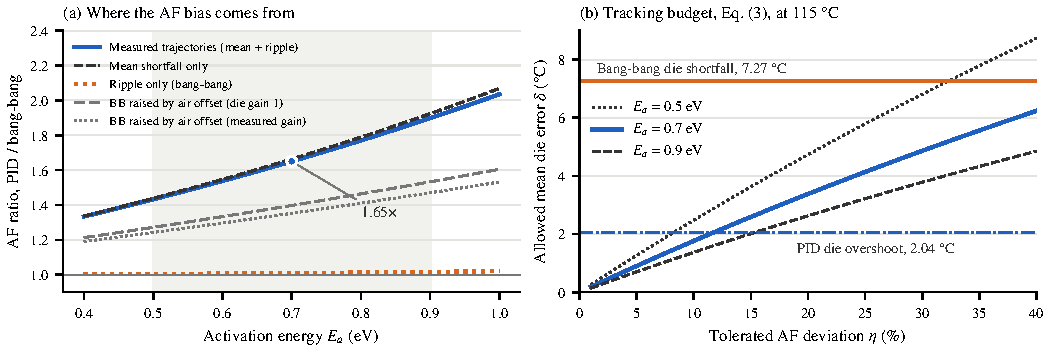
\includegraphics[width=\textwidth]{fig_stress.pdf}
\caption{Delivered stress on the \vDurPair-hour pair, from the measured die trajectories over each whole run. (a) PID-to-bang-bang ratio of $\langle AF\rangle$ versus activation energy: measured, mean shortfall only, ripple only, and with the bang-bang trajectory raised by the \vSPoffset\degC{} air offset (die gain 1, or the \vGainOLS{} measured on the long run). Shaded: common $E_a$ range. (b) Allowed mean die error, Eq.~\eqref{eq:delta}, versus tolerated AF deviation, with each bench's die error.}
\label{fig:stress}
\end{figure*}

The \vAFratio$\times$ ratio compares two bench architectures, not two thermostats on one loop. Only the PID bench closed a loop on the die; the die was logged on both. Its outer loop chose \vPIDspMax\degC{} of air, \vSPoffset\degC{} above the thermostat's 80\degC{} dial, and its supply was fixed rather than trimmed. If the thermostat held its dial and the die followed the air one-for-one, raising the thermostat by \vSPoffset\degC{} would still leave a \vAFratioSPadj$\times$ gap. The long run lets us test the second assumption: across 30-minute steps, the die moved \vGainOLS\degC{} per degree of air (an estimate instrumented by the setpoint moves, \vGainIV, is unstable in closed loop), which reduces the gap to \vAFratioSPgain$\times$; we cannot test the first. The die-to-air offset itself was not a constant of the oven: \vOffsetPID\degC{} on the 23-hour PID run and \vOffsetRCA\degC{} on the long run. A chamber setting therefore does not fix the die's mean, which is why the junction-referenced definition of JESD22-A108~\cite{jedec} needs die telemetry to verify. The XADC's absolute accuracy enters each bench's error against target but largely cancels in comparisons on the same chip.

% ---------------------------------------------------------------
\begin{figure*}[!t]
\centering
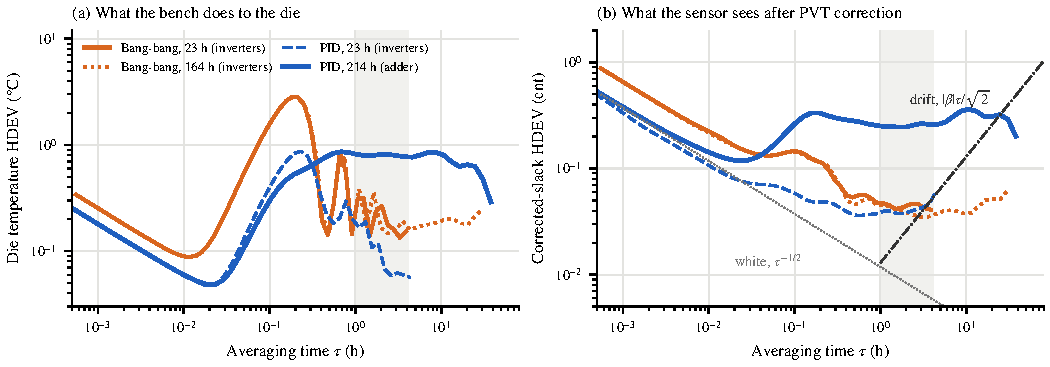
\includegraphics[width=\textwidth]{fig_allan.pdf}
\caption{Bench noise across averaging times, by overlapping Hadamard deviation (HDEV, insensitive to linear drift), first hour excluded, curves cut where fewer than about five windows remain. (a) Die temperature: the thermostat cycle peaks near \vCycleTauBB\,min; the long PID run wanders at hour scales. (b) PVT-corrected slack residual (regression on $T$ and $V$). Shaded: the 1--4\,h band used for the floor. Dash-dot: the long run's mean drift as an Allan line; dotted: white-noise slope.}
\label{fig:allan}
\end{figure*}

\section{Ripple averages out; slow wander does not}

Figure~\ref{fig:allan}(a) shows what each bench does to the die. The thermostat's cycle is a large bump, \vCyclePeakBB\degC{} near \vCycleTauBB\,min of averaging, and at the sampling interval it leaves a \vSigRawRatio$\times$ larger residual, \vSigRawBB{} against \vSigRawPID\,cnt~\cite{sbcci26} (\vSigRatio$\times$ for the fast residual, with the one-hour moving average removed; \vAdevTwoRatio$\times$ in Allan deviation at a common 2\,s). Figure~\ref{fig:allan}(b) shows that the correction removes almost all of this cycle: at the cycle's peak, \vRejPeakBB\% of its effect on the slack is gone. Lag between the XADC and the path is not the limit either; a heating-minus-cooling residual gap of \vHystBB\,cnt and a \vDtdtGainPct\% gain from a $dT/dt$ regressor rule it out.

Beyond an hour the picture changes. Both inverter-chain residuals flatten into a floor, \vFloorBB\,cnt on the bang-bang run and \vFloorPID\,cnt on the PID run (median HDEV over 1--4\,h), a \vFloorRatio$\times$ ratio; the \vDurBBlong-hour thermostatic log confirms the bang-bang floor (\vFloorBBlong\,cnt) over a week. The thermostat's sample-rate penalty thus shrinks at the averaging times that matter for aging. The long PID run, by contrast, sits on a floor of \vFloorRCA\,cnt. Its die wandered \vWanderRCA\degC{} at hour scales, \vWanderRatioBB$\times$ the thermostatic logs' \vWanderBBlong\degC: the outer loop, which acts only beyond $\pm3$\degC{} and in 1\degC{} steps every 30\,minutes, tolerates such wander by design. The PVT correction leaves a similar share of slow die wander on every run with enough of it: \vLeftBB\% on the 23-hour and \vLeftBBlong\% on the week-long thermostatic log, \vLeftRCA\% on the long PID run. Slow wander is corrected far less well than the fast cycle, presumably because the gradient between the XADC and the path changes slowly. The floor is therefore a property of the bench's slow thermal behavior, which a die-referenced loop sets as much as a thermostat does.

% ---------------------------------------------------------------
\begin{figure*}[!t]
\centering
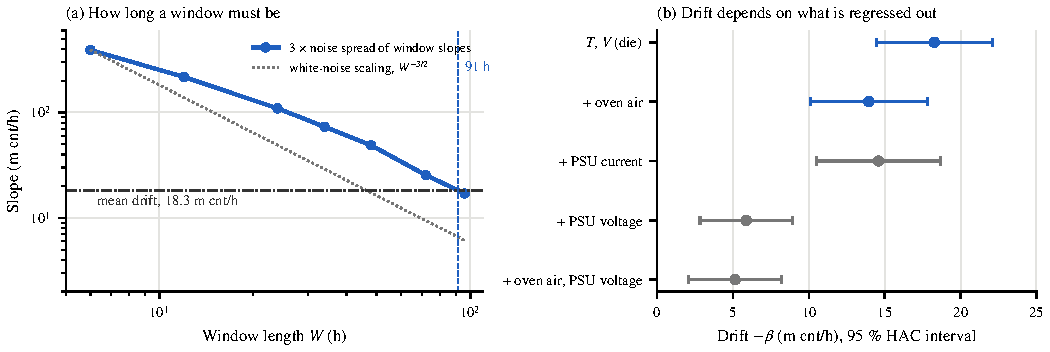
\includegraphics[width=\textwidth]{fig_drift.pdf}
\caption{The long PID run. (a) Spread of least-squares slopes of the corrected residual over sliding windows (2\,h stride), after removing the fitted power-law drift, versus window length; the drift is resolved at 3$\sigma$ where the spread meets the mean rate. (b) Drift (Newey--West errors on 10-minute block means, bandwidth 8\,h) for different regressor sets; gray sets include supply channels that drift at fixed die temperature and voltage.}
\label{fig:drift}
\end{figure*}

\section{How long until aging is visible}

\textbf{A sublinear drift is resolved.} After correction, the long run's residual drifts at \vBetaRCA\mcnth{} (95\% interval \vBetaLoRCA{} to \vBetaHiRCA), slowing from \vRCAfirstHalf{} to \vRCAsecondHalf\mcnth{} between halves; a power law $t^{n}$ with $n=\vPowNRCA$ fits 2-hour block means better than a line ($\Delta\mathrm{BIC}=\vdBICblockRCA$), as expected of bias-temperature instability. Time zero is the start of this run; the board's earlier stress makes $n$ an apparent exponent. The total, \vRCAdriftCnt\,cnt, is about \vRCAdriftPs\,ps of slack.

\textbf{Detection time.} With the fast residual ($\sigma=\vSigRCA$\,cnt, $\tint=\vTauRCA$\,s), Eq.~\eqref{eq:tmin} predicts \vTminBound\,h. The floor says otherwise, and three independent readings agree (Table~\ref{tab:tmin}). Figure~\ref{fig:allan}(b): the drift line crosses the floor at \vAllanCross-hour windows and reaches three times the two-window noise at \vAllanThree\,h, a \vAllanRun-hour run. Figure~\ref{fig:drift}(a): the spread of window slopes falls as $W^{-\vSdExpAbs}$, close to the floor regime's $W^{-1}$ and far from white noise's $W^{-3/2}$, and meets the mean drift at 3$\sigma$ for \vWstar-hour windows. Batch-means long-run variance at 8-hour blocks, substituted for $2\sigma^2\tint$ in Eq.~\eqref{eq:tmin}, gives \vTminLrv\,h.

\begin{table}[!t]
\centering
\caption{Time to resolve the long run's drift at 3$\sigma$, by method.}
\label{tab:tmin}
\footnotesize
\setlength{\tabcolsep}{2.5pt}
\begin{tabular}{@{}p{30mm} p{36mm} r@{}}
\toprule
Method & Noise model & Hours \\
\midrule
Eq.~\eqref{eq:tmin}, fast residual & white, $\sigma$ and $\tint$ & \vTminBound \\
Eq.~\eqref{eq:tmin}, long-run variance & wander up to 8\,h blocks & \vTminLrv \\
Window-slope spread & measured, drift law removed & \vWstar \\
Allan two-window & measured floor, Eq.~\eqref{eq:allan} & \vAllanRun \\
\bottomrule
\end{tabular}
\end{table} A day-long run cannot settle the question: slopes over \vWinLenMid-hour windows range from \vWinMinMid{} to $+$\vWinMaxMid\mcnth{}, and \vWinPosMid\% of them have the non-aging sign, whereas every \vWinLenLong-hour window is negative (\vWinMinLong{} to \vWinMaxLong). The nonzero late-window slopes that~\cite{sbcci26} found in both 23-hour runs therefore establish a drift within each run; whether it is aging needs the longer record.

\textbf{Which drift?} The rate depends on what is regressed out [Figure~\ref{fig:drift}(b)]: adding oven air gives \vBetaTVO, supply current \vBetaTVI, and supply voltage \vBetaTVP\mcnth. The supply channels fail the first rule of the primer. At fixed die temperature and voltage, the current rose by \vIdriftTotal\,mA and the supply voltage by \vPdriftTotal\,mV over the run, so both carry the device's state; the current is also \vCorrTIhourly-correlated with die temperature in hourly means, and adding either inflates the variance of the time coefficient \vVifTVI--\vVifTVP-fold. We therefore report \vBetaTVO{} to \vBetaRCA\mcnth{} from exogenous regressors and show the rest. The current also serves as a second, leakage-based thermometer: its drift at fixed XADC reading corresponds to only \vThermoShare\% of the temperature drift that would explain the slack drift, so a drifting XADC temperature reading cannot account for it, unless current aging cancels it. No logged channel isolates the clocking path.

\textbf{The bench penalty.} Under a floor, detection time scales roughly with floor/drift. On the 23-hour pair, the floor ratio is \vFloorRatio. The drift ratio depends on the aging law and on how much of the stress gap the thermostat alone owns: \vPenFloorAF$\times$ longer if drift scales with $\langle AF\rangle$ and the full \vAFratio$\times$ gap applies, \vPenFloorSP$\times$ with the setpoint-adjusted gap, and \vPenFloorPow$\times$ if drift follows the fitted power law in equivalent time. These ratios carry inverter-chain measurements to the adder, an assumption these data cannot test, and they hold the device's aging state fixed, which the paired runs did not.

% ---------------------------------------------------------------
\section{What labs should report}

The standards define the stress at the junction~\cite{jedec} or bound it there~\cite{mil}; what a sensor validation also needs is the noise at the right time scale. Table~\ref{tab:checklist} lists five items, each computable from a 1\,Hz log that includes die temperature, voltage, and the bench's actuator channels.

\begin{table}[!t]
\centering
\caption{Reporting checklist for sensor-instrumented burn-in, with values from this study.}
\label{tab:checklist}
\footnotesize
\setlength{\tabcolsep}{2.5pt}
\begin{tabular}{@{}p{28mm} p{55mm}@{}}
\toprule
Item & This study \\
\midrule
1. Die trajectory: mean, std.\ dev., error vs.\ target & BB \vTBB\,\textdegree C, \vTsdBB, \vTerrBB; PID \vTPID\,\textdegree C, \vTsdPID, $+$\vTerrPID \\
2. $\langle AF\rangle$ with $E_a$ range, and the loop that set the die & BB \vAFBB, PID \vAFPID{} at 0.7\,eV; ratio about \vAFratioLoOne--\vAFratioHiOne{} over 0.5--0.9\,eV \\
3. Allan/Hadamard deviation of $T$ and of the corrected residual & Floors \vFloorBB{} (BB), \vFloorPID{} (PID), \vFloorRCA\,cnt (long run) \\
4. Drift with its regressor set & \vBetaTVO{} to \vBetaRCA\mcnth{} (exogenous); \vBetaTVP{} with PSU voltage \\
5. Detection time, with method & Table~\ref{tab:tmin}: \vTminBound\,h (white) to \vAllanRun\,h (floor) \\
\bottomrule
\end{tabular}
\end{table}

\textbf{Limitations.} All data come from one 28\,nm board, so these are within-device results. The two circuits differ, and the paired runs were separate campaigns, with different oven setpoints, supply control, and device history. The stress (1.3--1.4\,V core, die near 125\degC) exceeds the device's absolute-maximum ratings: it is accelerated overstress chosen to make drift observable in days. Statements about JEDEC and MIL-STD conditions are interpretive.

% ---------------------------------------------------------------
% [SLOT: 16 nm FinFET transfer -- Artix UltraScale+ runs; go/no-go 2026-11-15]
% Keep commented out. The contingency version must compile and read complete
% without it. If enabled: one paragraph + at most one figure/table; add its
% numbers to analysis/ (new campaign key in dtlib.CAMPAIGNS) and to values.tex;
% re-run analysis/wordcount.py (budget headroom is printed there).
% \section{Transfer to a 16\,nm FinFET FPGA}
% ...
% ---------------------------------------------------------------

% Closing (CEDA: 1-2 paragraphs, lessons learned and future rather than a summary)
\section{Conclusion}

The lesson for anyone validating an on-chip sensor under burn-in is to look at the bench through the sensor's averaging time. The bench's mean die temperature sets the stress, and only die telemetry verifies it. Its fast ripple, the most visible symptom of a thermostat, is largely removed by a PVT correction; its slow die wander is not, and that wander set a detection time of about \vWstar\,h where a white-noise model promised \vTminBound. A die-referenced loop fixes the mean, but with a coarse outer step it can raise the floor it is meant to lower.

Three steps follow. A finer, continuous die loop should lower the floor, and the Allan plot will show by how much. A reference path that does not age, or a second sensor, would separate readout from device drift. Replication across boards, and on a 16\,nm FinFET FPGA, would turn these within-device results into population statistics.

% ---------------------------------------------------------------
\renewcommand{\refname}{References}\begin{thebibliography}{12}
\footnotesize
\bibitem{kashyap} R.~Kashyap, ``Silicon lifecycle management (SLM) with in-chip monitoring,'' in \emph{Proc. IEEE Int. Rel. Phys. Symp. (IRPS)}, 2021, pp.~1--4, doi: 10.1109/IRPS46558.2021.9405187.
\bibitem{niemann} C.~Niemann, M.~Ali, O.~U.~Shah, J.~Heller, and D.~Timmermann, ``Sensor based adaptive voltage scaling on FPGAs: Calibration and parametrization,'' \emph{Integration}, vol.~75, pp.~30--39, 2020, doi: 10.1016/j.vlsi.2020.05.006.
\bibitem{valdes} M.~Vald\'es-Pe\~na \emph{et al.}, ``Design and validation of configurable online aging sensors in nanometer-scale FPGAs,'' \emph{IEEE Trans. Nanotechnol.}, vol.~12, no.~4, pp.~508--517, 2013, doi: 10.1109/TNANO.2013.2253795.
\bibitem{jedec} \emph{Temperature, Bias, and Operating Life}, JEDEC Standard JESD22-A108G, 2022.
\bibitem{mil} \emph{Environmental Test Methods for Microcircuits, Part~1: Test Methods 1000--1999}, MIL-STD-883-1, Method 1015: Burn-In Test, U.S. Department of Defense, 2019.
\bibitem{vassighi} A.~Vassighi, O.~Semenov, M.~Sachdev, A.~Keshavarzi, and C.~Hawkins, ``CMOS IC technology scaling and its impact on burn-in,'' \emph{IEEE Trans. Device Mater. Rel.}, vol.~4, no.~2, pp.~208--221, 2004, doi: 10.1109/TDMR.2004.826591.
\bibitem{sobas} J.~Sobas, T.-B.~Airimitoaie, and F.~Marc, ``Development of a high accuracy and stability test bench for ageing measurement of 16\,nm FinFETs based FPGA,'' \emph{Microelectron. Rel.}, vol.~138, 2022, Art. no.~114698, doi: 10.1016/j.microrel.2022.114698.
\bibitem{sbcci26} D.~Alencar \emph{et al.}, ``Quantifying the effect of burn-in thermal control on delivered acceleration factor and on-chip slack-sensor fidelity in an FPGA target,'' in \emph{Proc. 39th Symp. Integr. Circuits Syst. Design (SBCCI)}, 2026, to be published.
\bibitem{sbcci25} L.~Nogueira \emph{et al.}, ``Auto-tuning aging sensor validated under burn-in, temperature, and voltage variations,'' in \emph{Proc. 38th Symp. Integr. Circuits Syst. Design (SBCCI)}, 2025, pp.~1--5.
\bibitem{simc} S.~Skogestad, ``Simple analytic rules for model reduction and PID controller tuning,'' \emph{J. Process Control}, vol.~13, no.~4, pp.~291--309, 2003.
\bibitem{allan} D.~W.~Allan, ``Statistics of atomic frequency standards,'' \emph{Proc. IEEE}, vol.~54, no.~2, pp.~221--230, 1966, doi: 10.1109/PROC.1966.4634.
\bibitem{weatherhead} E.~C.~Weatherhead \emph{et al.}, ``Factors affecting the detection of trends: Statistical considerations and applications to environmental data,'' \emph{J. Geophys. Res.}, vol.~103, no.~D14, pp.~17149--17161, 1998, doi: 10.1029/98JD00995.
\end{thebibliography}

% ---------------------------------------------------------------
% Biographies (CEDA: position, highest degree, discipline, institution, <= 3 interests, memberships, e-mail)
\section*{Author Biographies}
\footnotesize
\noindent\textbf{Danilo Alencar} is a master's student in teleinformatics engineering at the Universidade Federal do Cear\'a (UFC), Fortaleza, Brazil, and a researcher at the Laboratory of Electronic Systems and Circuits (LESC). His research interests include FPGA reliability, aging instrumentation, and silicon lifecycle management. Alencar has a BSc in computer engineering from UFC. Contact him at danilo.alencar@lesc.ufc.br.

\smallskip\noindent\textbf{Lucas Nogueira} is with LESC, UFC, Fortaleza, Brazil. His research interests include on-chip aging sensors and FPGA delay monitoring. Contact him at lucas.nogueira@lesc.ufc.br.

% TODO(authors): complete co-author bios per CEDA (position, highest degree + discipline + institution, <=3 interests, memberships, e-mail)
\smallskip\noindent\textbf{Alisson Barros}, \textbf{Arthur Pamplona}, and \textbf{Andre Grangeiro} are with LESC, UFC, Fortaleza, Brazil. Their research interests include FPGA test platforms and reliability instrumentation.

\smallskip\noindent\textbf{Jarbas Silveira} is a professor at UFC, Fortaleza, Brazil, and leads research at LESC. His research interests include integrated-circuit design, test, and reliability. Contact him at jarbas@lesc.ufc.br.

\smallskip\noindent\textbf{Fabian Vargas} is with IHP -- Leibniz Institute for High Performance Microelectronics, Frankfurt (Oder), Germany. His research interests include on-chip sensors, design for reliability, and silicon lifecycle management. Contact him at vargas@ihp-microelectronics.com.

\medskip\noindent Direct questions and comments about this article to Danilo Alencar, Laboratory of Electronic Systems and Circuits (LESC), Universidade Federal do Cear\'a, Fortaleza, CE, Brazil; danilo.alencar@lesc.ufc.br.

\end{document}
